
\documentclass[12pt]{article}
\usepackage{amsmath}
\usepackage{geometry}
\usepackage{chngcntr}
\usepackage{graphicx}
\usepackage{authblk}
\usepackage{caption}
 \usepackage{lineno}
 \usepackage{blindtext}

\newcommand{\absdiv}[1]{%
  \par\addvspace{.5\baselineskip}% adjust to suit
  \noindent\textbf{#1}\quad\ignorespaces
}

\geometry{margin=1.25in}
\captionsetup{width=5in}


\title{Overview of MRI Environment}
\author[]{Nikolai Mickevicius, Ph.D.}

\affil[]{Department of Biophysics, Medical College of Wisconsin}

\date{}

\begin{document}
% \linenumbers

\maketitle

\abstract{

\absdiv{Outline}

\begin{enumerate}
    \item What makes MRI special?
    \item The MRI Exam
    \item MRI scanner hardware
\end{enumerate}

\newpage

\section{What makes MRI special?}

Consider your smartphone camera. It uses small lenses to focus light reflected off your subject on a sensor. That sensor contains millions of photodiodes that convert the light into an electrical signal that is digitized. Each pixel in an image corresponds to a unique sensor. 

In radiographic imaging, x-ray radiation (with a wavelengths near $0.01$ nm) is attenuated as it interacts with the molecules in your body. Similar to camera sensors, each pixel of an x-ray image is its own individual element of a detector array. 

Computed tomography uses a spinning x-ray machine to reconstruct 3D images using digital radiographs acquired at many angles around the patient. Thus, it requires 1) many thousands of detector elements, 2) extremely small wavelengths of radiation (high energy and ionizing), and 3) moving parts to generate a diagnostic 3D image. 

Magnetic Resonance Imaging (MRI): Making images with millimeter resolution using electromagnetic energy with a wavelength longer than the human body \emph{with no moving parts and a single detector element}. It does so using radio waves very close to the FM stations (128 MHz for 3T systems versus upper end of 108.0 MHz for FM radio). This corresponds to wavelengths of
\begin{equation}
    \lambda = \frac{c}{f}=\frac{3.0 \times 10^8\text{\ m/s}}{1.28 \times 10^8\text{\ Hz}}=2.34\text{\ m}.
\end{equation}
Further, the signal from which images can be created can be collected with even a single detector element (compared with the thousands or millions needed for other medical imaging modalities). 

In this course, you will learn the beautiful physics of how this is possible and how the contrast of an image can be manipulated to see specific diseases, microscopic tissue structure, and even physiological function. 

\section{The MRI Exam}

\noindent\textbf{Overview.} An MRI appointment typically lasts 20--60 minutes, depending on the body part and the number of image ``sequences'' (scan types) required. The experience follows a predictable workflow designed to maximize safety, comfort, and image quality.

\medskip
\noindent\textbf{1) Safety screening.} Before entering the scan room, you will complete a detailed questionnaire and speak with MRI staff. The goal is to identify any implanted or external items that could move, heat, malfunction, or distort images in the strong magnetic field. Common topics include cardiac devices, aneurysm clips, cochlear implants, medication patches, insulin pumps, neurostimulators, metal fragments (especially from prior injuries or surgeries), dental hardware, cosmetic tattoos, and pregnancy. In some cases, documentation about an implant is required to confirm MRI compatibility.

\medskip
\noindent\textbf{2) Removing metal.} Because the static magnetic field is always on, all loose metallic objects must be removed: phones, wallets, keys, coins, watches, jewelry, hairpins, fitness trackers, hearing aids, credit cards, and clothing with metallic fibers, snaps, or zippers. Makeup with metallic pigments and some transdermal patches can also be problematic. Lockers are usually provided, and facilities often supply MRI-safe clothing.

\medskip
\noindent\textbf{3) Positioning on the table.} A technologist will help you lie on a padded table in a specific position (supine is most common). Specialized radiofrequency (RF) ``coils'' that both transmit and receive signals are placed around or near the area being imaged (e.g., a head coil like a helmet, a body coil over the abdomen, or small flexible coils for joints). Soft pads and straps may be used to minimize motion and keep you comfortable. You will receive a call button to alert staff at any time.

\medskip
\noindent\textbf{4) Inside the bore: space and airflow.} The table slides into the scanner's bore (a cylindrical opening). The space can feel close, particularly for head or spine exams. Modern systems provide fans for airflow and small mirrors or periscopes so you can see out; some facilities offer music, video goggles, or ambient lighting. If you are prone to claustrophobia, tell the staff beforehand—options include extra coaching, a support person in the room (when safe), short breaks between sequences, use of a wider-bore scanner, or prescribed anxiolytic medication arranged in advance.

\medskip
\noindent\textbf{5) Sounds and ear protection.} During image acquisition, rapidly switching gradient coils produce loud tapping or thumping noises. You will be given earplugs, earmuffs/headphones, or both; with protection, sound levels are reduced to safe ranges. The technologist maintains two-way communication and will announce when each sequence starts and how long it will last.

\medskip
\noindent\textbf{6) Staying still and following instructions.} Image sharpness depends on minimizing motion. Expect to remain as still as possible and, for some exams (e.g., chest or abdomen), to perform brief breath-holds. Between sequences the table may move slightly, or the technologist may make minor adjustments to coils or padding.

\medskip
\noindent\textbf{7) Intravenous contrast (when indicated).} Some studies require a gadolinium based contrast agent (GBCA) given through a small IV, often placed in the hand or arm before you enter the room. The injection typically occurs mid-exam and may cause a transient cool or warm sensation or a mild metallic taste. Contrast helps highlight blood vessels, tumors, inflammation, and post-surgical changes by altering tissue signal on certain sequences. Adverse reactions are uncommon; severe reactions are rare. Because most GBCAs are cleared by the kidneys, patients with significantly reduced kidney function may undergo additional screening or receive specific agents according to institutional policy.

\medskip
\noindent\textbf{8) After the scan and getting results.} When imaging is complete, the technologist removes coils and IV (if placed) and helps you off the table. You can usually resume normal activities immediately unless instructed otherwise (e.g., after sedation). Images are interpreted by a radiologist, who sends a report to your ordering clinician. Turnaround times vary by site and urgency; routine outpatient results are commonly available within one to three business days. Your clinician will discuss findings and next steps.

\medskip
\noindent\textbf{Practical tips for patients.} Wear simple, metal-free clothing; bring implant information cards; arrive early for screening; and let staff know about claustrophobia, pain, or difficulty lying flat. Good communication with the technologist is the single best predictor of a smooth exam and high-quality images.


\section{MRI scanner hardware}

\subsection{Static magnetic field}

The main field $B_0$ defines the \emph{polarization axis}—the direction along which nuclear spins slightly align (conventionally $\hat{z}$). The Larmor frequency scales with field strength, $f_0=\gamma B_0/2\pi$, and higher $B_0$ increases net magnetization and thus SNR. (We will get much more into this in later lectures.) Clinically common values are $1.5$~T and $3$~T, while research systems reach $7$~T and above. For reference, Earth’s field is $\sim 50~\mu\mathrm{T}$, so a $3$~T magnet is $\sim 60{,}000\times$ stronger. At these field strengths the main magnets are superconducting solenoids operated near $4$~K in a helium cryostat (often with cryocoolers) and run in persistent mode for exceptional temporal stability; the magnet is \emph{always on}. Modern designs also use actively shielded windings to confine the fringe field without compromising the uniformity of $B_0$ in the imaging volume.


\paragraph{Homogeneity and stability.}
Image quality and spectroscopy demand an extremely uniform $B_0$ within a ``diameter spherical volume'' (DSV) centered at isocenter. Modern systems achieve sub‐ppm homogeneity over head/torso volumes using a combination of passive shims (small pieces of ferromagnetic material placed during installation) and active shim coils (auxiliary low‐current coils) that generate corrective fields. After shimming, temporal drift is minimized by operating the magnet in \emph{persistent mode} (superconducting loop closed by a superconducting switch), yielding very low frequency drift over time.

\paragraph{Shielding and fringe field.}
MRI magnets are typically air‐core, superconducting solenoids. To reduce the extent of the fringe field (the field outside the bore), many systems use \emph{active shielding}: secondary coils carrying opposing current confine $B$ outside the scanner while minimally perturbing $B_0$ inside. Site planning is based on the \emph{5‐gauss (0.5 mT) line}, beyond which ferromagnetic items and certain medical devices (e.g., many legacy cardiac implants) must not enter. When you enter MRI Zone IV (the room where the scanner actually resides), you will see the 5-gauss line indicated on the floor. 

\paragraph{Safety notes (static field).}
The static field is always on. Translational force on ferromagnetic objects scales with $B\nabla B$ and torque with $\boldsymbol{\tau}=\mathbf{m}\times\mathbf{B}$, producing the projectile hazard and implant rotation risk. Screening and controlled access (Zones I–IV) mitigate these hazards. In a magnet \emph{quench} (loss of superconductivity), liquid helium rapidly boils off; quench pipes vent gas to the outside, but oxygen monitoring and emergency procedures are critical for room safety. Although, latest generation scanners (2025 and newer) are completely sealed, require only 0.7 L of liquid helium, and may not even have a quench pipe. 

\subsubsection{Magnetic field in a solenoid}
In the Biot--Savart law,
\[
\mathbf{B}(\mathbf{r})=\frac{\mu_0}{4\pi}\int \frac{I\, d\boldsymbol{\ell}'\times\mathbf{R}}{R^3},
\qquad
\mathbf{R}=\mathbf{r}-\mathbf{r}',\quad R=\lVert\mathbf{R}\rVert,
\]
\emph{unprimed} quantities (e.g., $\mathbf{r}$) refer to the \textbf{observation point} where the field is evaluated, while \emph{primed} quantities (e.g., $\mathbf{r}'$, $d\boldsymbol{\ell}'$) refer to the \textbf{source point} along the current path being integrated over. The prime simply reminds us that $\mathbf{r}'$ is a dummy variable of integration that runs over the wire. The vector $d\boldsymbol{\ell}'$ is the differential line element \emph{tangent} to the wire at $\mathbf{r}'$ and oriented with the current direction; the product $I\,d\boldsymbol{\ell}'$ is the elemental ``current segment.''

\paragraph{Field on the axis of a circular current loop}
Take a loop of radius $a$ in the $x$--$y$ plane (center at the origin) carrying current $I$ in the $+\hat{\boldsymbol{\phi}}$ direction. Parameterize the \emph{source} point by the azimuthal angle $\phi$:
\[
\mathbf{r}'(\phi)=a\cos\phi\,\hat{\mathbf{x}}+a\sin\phi\,\hat{\mathbf{y}},\qquad
d\boldsymbol{\ell}'=\frac{d\mathbf{r}'}{d\phi}\,d\phi
=\big(-a\sin\phi\,\hat{\mathbf{x}}+a\cos\phi\,\hat{\mathbf{y}}\big)\,d\phi
= a\,d\phi\,\hat{\boldsymbol{\phi}}.
\]
Place the \emph{observation} point on the axis at $\mathbf{r}=z_0\,\hat{\mathbf{z}}$. Then
\[
\mathbf{R}=\mathbf{r}-\mathbf{r}'=z_0\,\hat{\mathbf{z}}-a\cos\phi\,\hat{\mathbf{x}}-a\sin\phi\,\hat{\mathbf{y}}
= z_0\,\hat{\mathbf{z}}-a\,\hat{\boldsymbol{\rho}},\qquad
R=\sqrt{a^2+z_0^2}.
\]
The cross product appearing in Biot--Savart simplifies neatly:
\[
d\boldsymbol{\ell}'\times\mathbf{R}
= a\,d\phi\,\hat{\boldsymbol{\phi}}\times\big(z_0\,\hat{\mathbf{z}}-a\,\hat{\boldsymbol{\rho}}\big)
= a\,d\phi\big(z_0\,\hat{\boldsymbol{\rho}}+a\,\hat{\mathbf{z}}\big).
\]
When integrated over $\phi\in[0,2\pi)$, the $\hat{\boldsymbol{\rho}}$ contributions cancel by symmetry (their vector average around the ring is zero), leaving only the axial component. Therefore,
\[
B_z(z_0)=\frac{\mu_0}{4\pi}\int_0^{2\pi}\frac{I\,(a^2\,d\phi)}{(a^2+z_0^2)^{3/2}}
=\frac{\mu_0 I a^2}{2\left(a^2+z_0^2\right)^{3/2}},
\]
which is the standard on-axis field of a circular loop.


\paragraph{Long-solenoid limit.}
For $L\gg a$,
\[
\frac{L}{\sqrt{a^2+\left(\tfrac{L}{2}\right)^2}}\to 2
\quad\Rightarrow\quad
\boxed{\,B_z \xrightarrow{L\gg a} \mu_0 n I\,},
\]
recovering the familiar uniform-field result inside an ideal long solenoid. This Biot--Savart derivation also makes clear how edge effects (\emph{fringe field}) arise near the ends via the finite-$L$ terms.

\medskip
\noindent\emph{Note.} Off-axis fields of a single loop can be expressed using complete elliptic integrals; in practice, MRI main-magnet windings are designed (often with multiple coaxial coil sets) to minimize off-axis inhomogeneity within the imaging DSV while controlling the external fringe field.

\subsection{Gradient coils}

Nested within the solenoid coil producing the strong static field are three additional coils that change $B_z$ as a linear function of $x$, $y$, and $z$. 
\begin{equation}
    B_z = B_0 + G_x x + G_y y + G_z z
\end{equation}
Again, I want to emphasize that $G_x$ produces a \emph{pointing along} $\hat{z}$ that varies as a function of $x$. It does not point along $\hat{x}$! 



\paragraph{Constructing a $z$ Gradient.}
For a single loop of radius $a$ centered at $z=z_0$, the on-axis field is
\[
B_z^{\text{loop}}(z;z_0,I)=\frac{\mu_0 I a^2}{2\big(a^2+(z-z_0)^2\big)^{3/2}}.
\]
Now place two identical coaxial loops at $z=\pm d/2$ with equal and opposite currents ($+I$ at $+d/2$, $-I$ at $-d/2$). The superposed on-axis field is
\[
\boxed{\,B_z(z)=\frac{\mu_0 I a^2}{2}\!\left[
\frac{1}{\big(a^2+(z-\tfrac{d}{2})^2\big)^{3/2}}
-\frac{1}{\big(a^2+(z+\tfrac{d}{2})^2\big)^{3/2}}
\right].\,}
\]
(For $N$ turns per loop, multiply by $N$.)

\paragraph{Odd symmetry and zero field at the center.}
Let $F(u)=\big(a^2+u^2\big)^{-3/2}$, which is an even function: $F(-u)=F(u)$. Then
\[
B_z(z)=\frac{\mu_0 I a^2}{2}\,\big[F(z-\tfrac{d}{2})-F(z+\tfrac{d}{2})\big]
\]
is an \emph{odd} function of $z$, so $B_z(0)=0$.

\paragraph{Linearization about the center.}
Taylor expand $F$ about $u=\tfrac{d}{2}$:
\[
F(z\!\mp\!\tfrac{d}{2})=F(u)\mp z F'(u)+\frac{z^2}{2}F''(u)\mp\frac{z^3}{6}F^{(3)}(u)+\cdots.
\]
Subtracting,
\[
F(z-\tfrac{d}{2})-F(z+\tfrac{d}{2})=2zF'(u)+\frac{z^3}{3}F^{(3)}(u)+\mathcal{O}(z^5).
\]
Since $F'(u)=-3u\big(a^2+u^2\big)^{-5/2}$ with $u=\tfrac{d}{2}$, the leading term is linear:
\[
\boxed{\,B_z(z)\approx G\,z,\qquad
G=\left.\frac{dB_z}{dz}\right|_{z=0}
=\frac{3\mu_0 I a^2 d}{2\big(a^2+(\tfrac{d}{2})^2\big)^{5/2}}.\,}
\]
The next nonzero correction is cubic in $z$ (the quadratic term cancels by symmetry), so for $|z|\ll a$ the field is approximately linear over a central region. Choosing $d$ relative to $a$ can further suppress higher-order terms to enlarge this linear region (a classic design goal in gradient coils).


\begin{figure}[h]
    \centering
    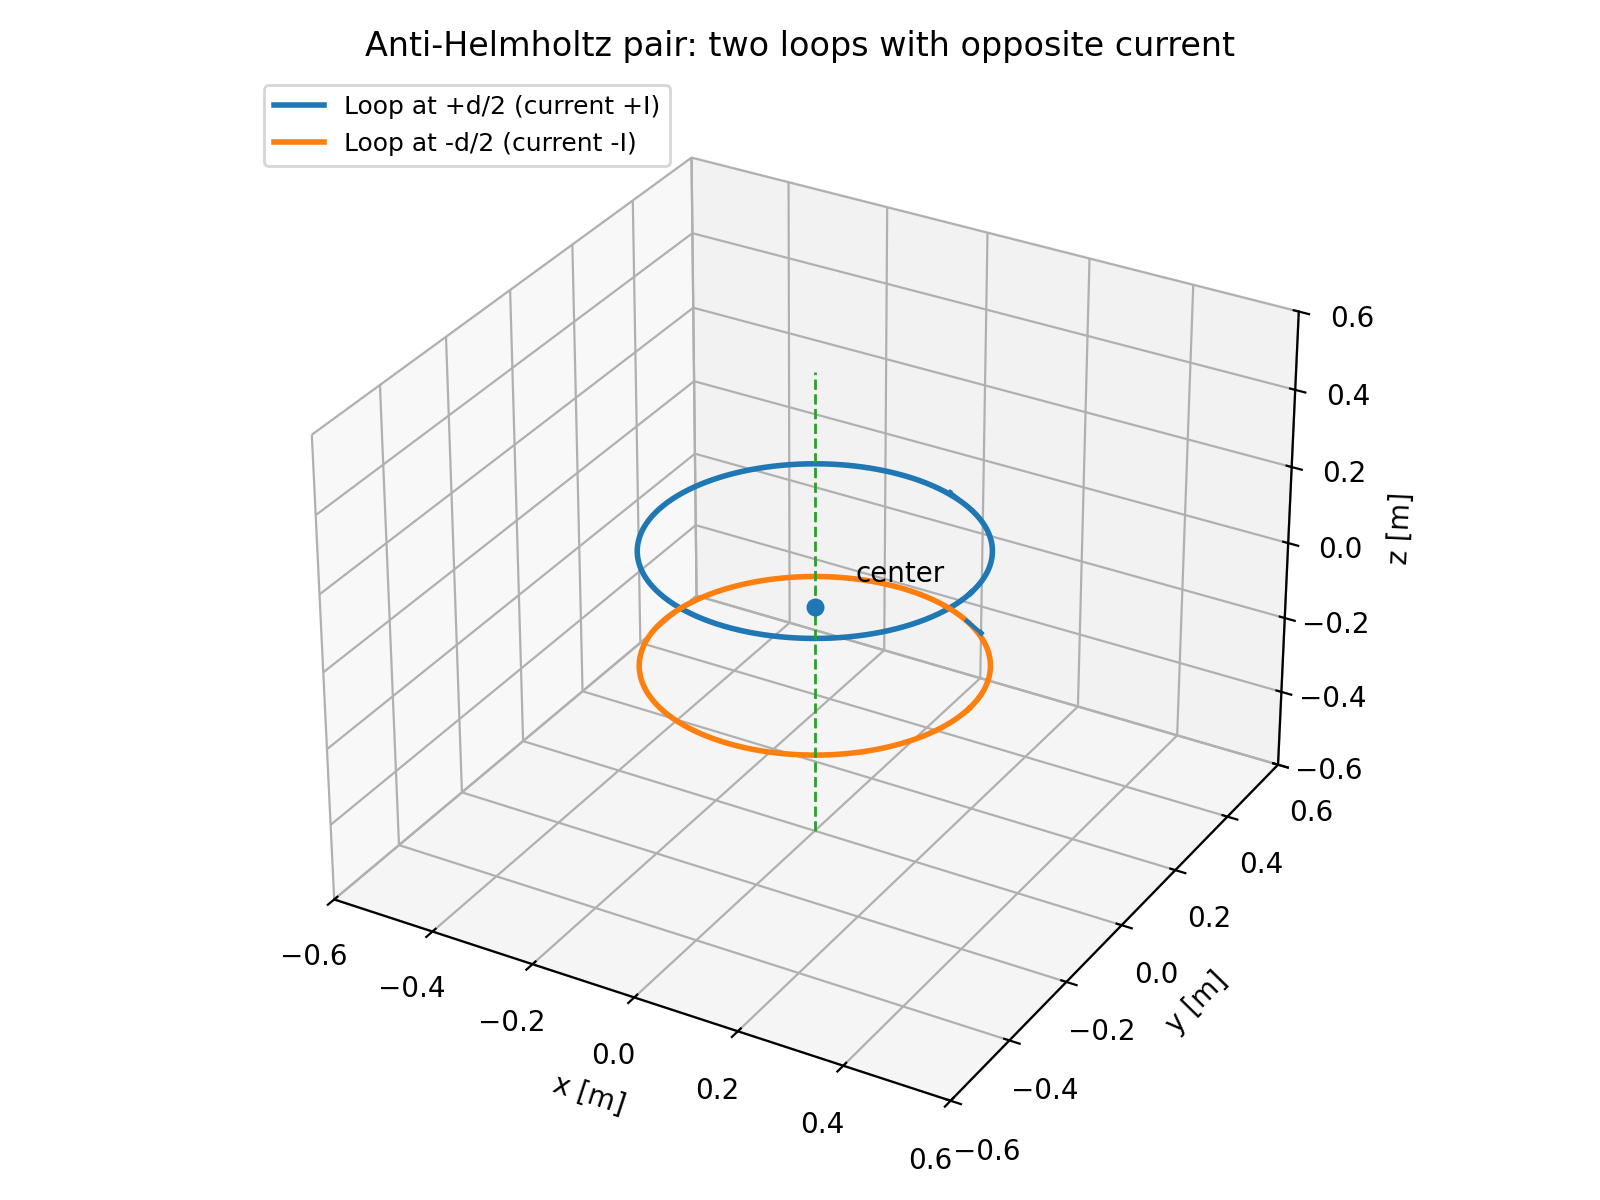
\includegraphics[width=0.6\textwidth]{antihelmholtz_geometry.png}
    \caption{Two current loops with radii of $a$ and opposite current direction are spaced a distance $d$ apart. This geometry was used to derive the equation for the $z$ gradient.}
    \label{fig:gz_setup}
\end{figure}


\begin{figure}[h]
    \centering
    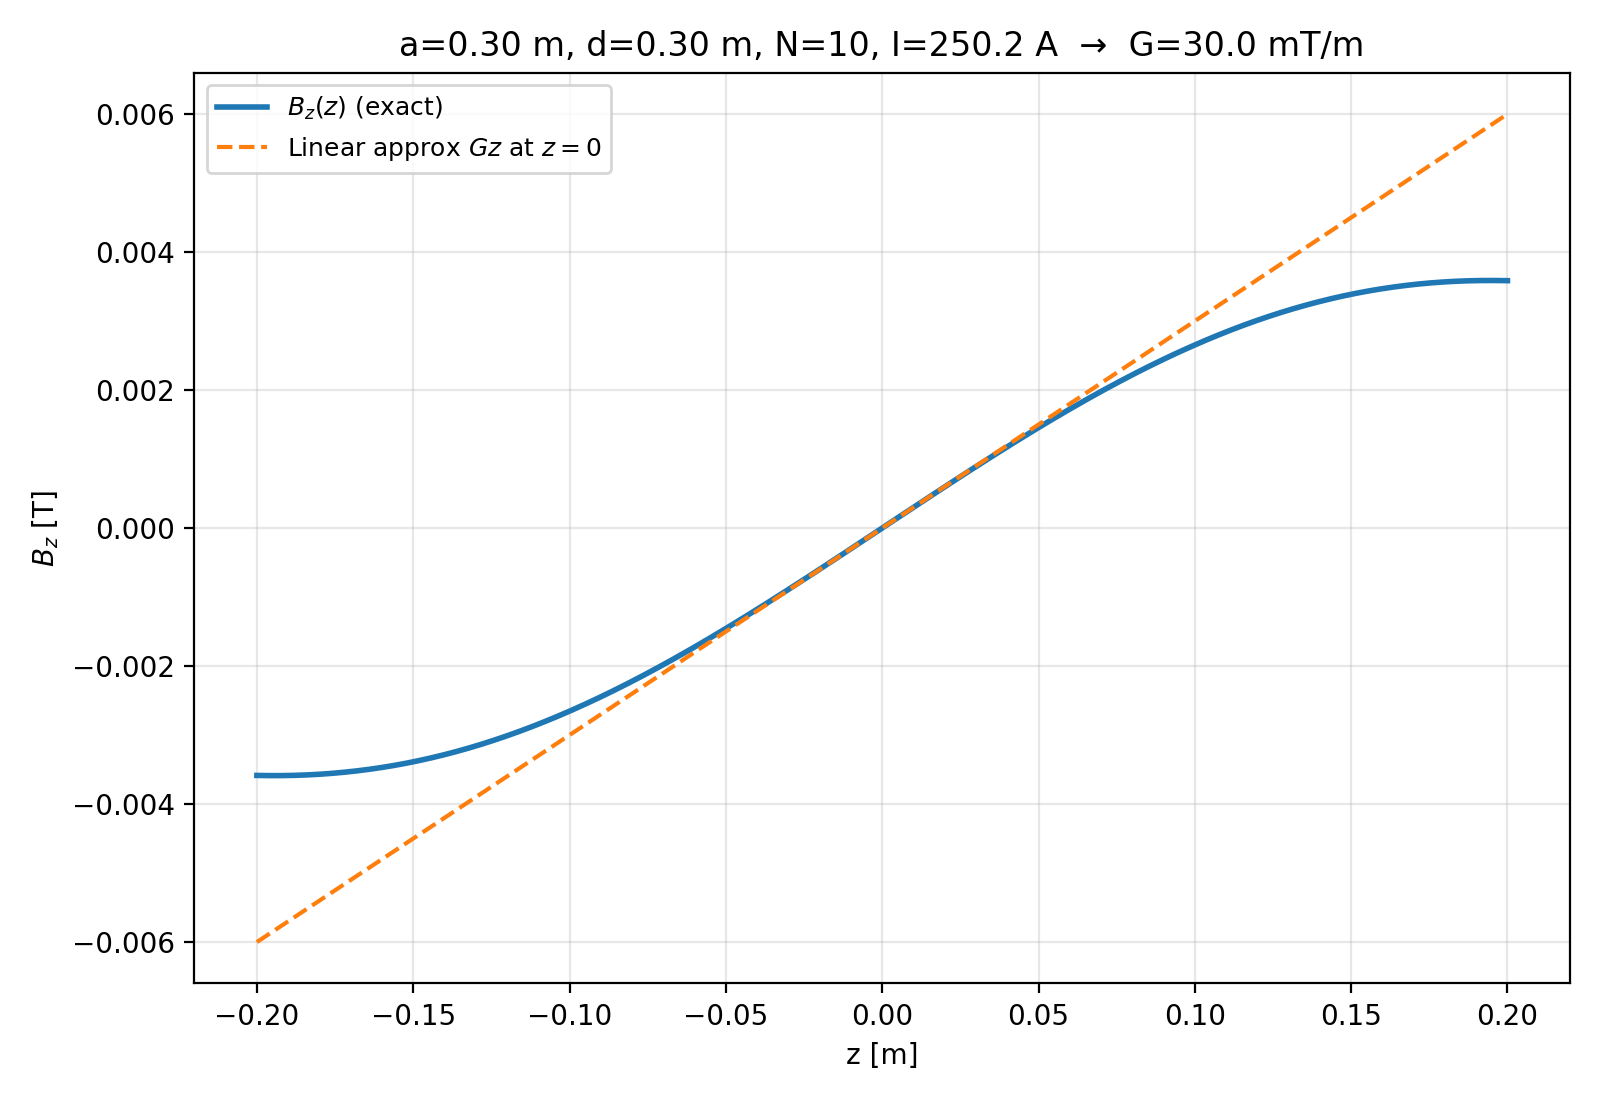
\includegraphics[width=0.6\textwidth]{antihelmholtz_Bz_vs_z.png}
    \caption{Plot of $B_z(z)$ for our simple gradient coil consisting of two current loops.}
    \label{fig:gz_setup}
\end{figure}

\newpage

\subsection{Radiofrequency coils}

We have discussed $B_0$ including the static field and additional gradients that we superimpose on it. However, there is another key component of an MRI system, namely, radiofrequency coils. These coils \emph{do} produce fields in the $x$ and $y$ directions, which we call $B_1$ fields. RF energy is passed through the coil in order to "excite" the nuclear spins in the subject in order to make their signal "visible". The same coil used to transmit RF energy to the subject can also be used to receive the RF signal that is generated by the subject.  

\subsection{Birdcage RF Transmit Coil}

The birdcage coil design (see python script) is built into the bore of the scanner. It produces an exceptionally uniform $B_1$ field, making it ideal for excitation of spins. It is often driven in quadrature, meaning RF energy is fed in with both 0$^\circ$ and 90$^\circ$ phase, producing circularly polarized fields along $x$ and $y$. 

\subsection{Phased Array Coils}

While only a single detector is theoretically necessary to gather all the data needed to make an image, it is more practical to use separate coils far closer to the subject (to improve signal-to-noise ratio). There are typically 12-64 individual receiver elements contained in an array. Each element consists of  a small loop of wire ~4 cm in diameter with a capacitor tuned to match the circuit to the resonant frequency of the scanner (i.e., 128 MHz at 3T). 

\begin{figure}[h]
    \centering
    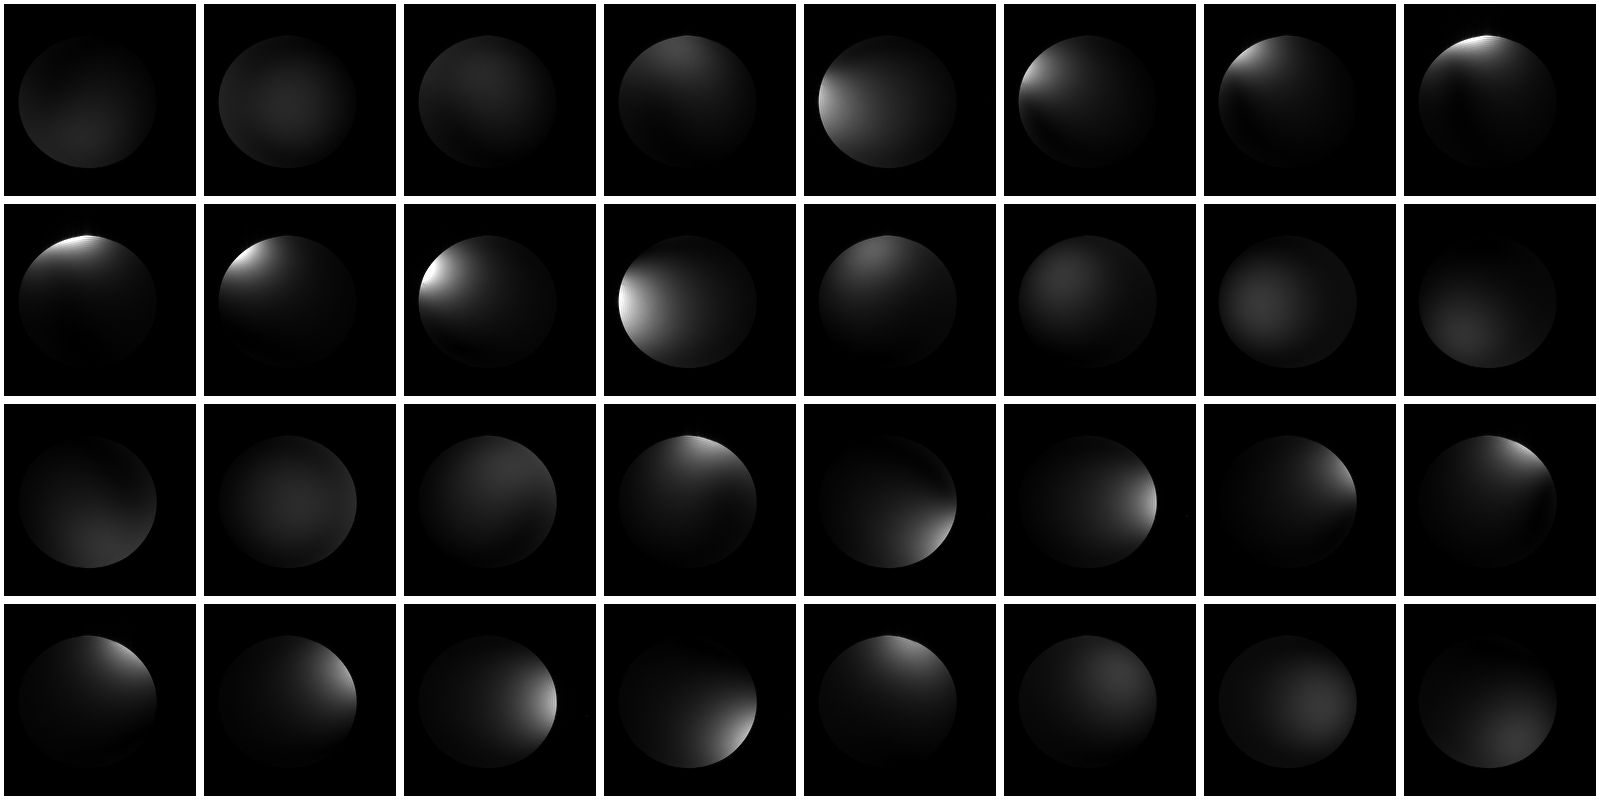
\includegraphics[width=0.8\textwidth]{coil_images.png}
    \caption{Images from each of the 32 elements of a head coil commonly used at MCW Center for Imaging Research.}
    \label{fig:coil_images}
\end{figure}

\end{document}